
%% bare_conf.tex
%% V1.3
%% 2007/01/11
%% by Michael Shell
%% See:
%% http://www.michaelshell.org/
%% for current contact information.
%%
%% This is a skeleton file demonstrating the use of IEEEtran.cls
%% (requires IEEEtran.cls version 1.7 or later) with an IEEE conference paper.
%%
%% Support sites:
%% http://www.michaelshell.org/tex/ieeetran/
%% http://www.ctan.org/tex-archive/macros/latex/contrib/IEEEtran/
%% and
%% http://www.ieee.org/

%%*************************************************************************
%% Legal Notice:
%% This code is offered as-is without any warranty either expressed or
%% implied; without even the implied warranty of MERCHANTABILITY or
%% FITNESS FOR A PARTICULAR PURPOSE! 
%% User assumes all risk.
%% In no event shall IEEE or any contributor to this code be liable for
%% any damages or losses, including, but not limited to, incidental,
%% consequential, or any other damages, resulting from the use or misuse
%% of any information contained here.
%%
%% All comments are the opinions of their respective authors and are not
%% necessarily endorsed by the IEEE.
%%
%% This work is distributed under the LaTeX Project Public License (LPPL)
%% ( http://www.latex-project.org/ ) version 1.3, and may be freely used,
%% distributed and modified. A copy of the LPPL, version 1.3, is included
%% in the base LaTeX documentation of all distributions of LaTeX released
%% 2003/12/01 or later.
%% Retain all contribution notices and credits.
%% ** Modified files should be clearly indicated as such, including **
%% ** renaming them and changing author support contact information. **
%%
%% File list of work: IEEEtran.cls, IEEEtran_HOWTO.pdf, bare_adv.tex,
%% bare_conf.tex, bare_jrnl.tex, bare_jrnl_compsoc.tex
%%*************************************************************************

% *** Authors should verify (and, if needed, correct) their LaTeX system ***
% *** with the testflow diagnostic prior to trusting their LaTeX platform ***
% *** with production work. IEEE's font choices can trigger bugs that do ***
% *** not appear when using other class files. ***
% The testflow support page is at:
% http://www.michaelshell.org/tex/testflow/



% Note that the a4paper option is mainly intended so that authors in
% countries using A4 can easily print to A4 and see how their papers will
% look in print - the typesetting of the document will not typically be
% affected with changes in paper size (but the bottom and side margins will).
% Use the testflow package mentioned above to verify correct handling of
% both paper sizes by the user's LaTeX system.
%
% Also note that the "draftcls" or "draftclsnofoot", not "draft", option
% should be used if it is desired that the figures are to be displayed in
% draft mode.
%
\documentclass[conference]{IEEEtran}
% Add the compsoc option for Computer Society conferences.
%
% If IEEEtran.cls has not been installed into the LaTeX system files,
% manually specify the path to it like:
% \documentclass[conference]{../sty/IEEEtran}

\usepackage{graphicx}
\usepackage{datetime}
\usepackage{cite}
\usepackage[hyphens]{url}
\usepackage[hidelinks]{hyperref}
\usepackage{csquotes}
\usepackage{array}
\usepackage {adjustbox}
\usepackage{tcolorbox}
\usepackage{graphicx}
\usepackage{multirow}
\usepackage{multicol}
\usepackage{pdflscape}
\usepackage{amsmath}
\usepackage{float}
\usepackage{afterpage}
\graphicspath{ {images/} }
\hypersetup{breaklinks=true}
\newcommand{\subparagraph}{}
\usepackage{titlesec}
\setcounter{secnumdepth}{4}

% Some very useful LaTeX packages include:
% (uncomment the ones you want to load)


% *** MISC UTILITY PACKAGES ***
%
%\usepackage{ifpdf}
% Heiko Oberdiek's ifpdf.sty is very useful if you need conditional
% compilation based on whether the output is pdf or dvi.
% usage:
% \ifpdf
% % pdf code
% \else
% % dvi code
% \fi
% The latest version of ifpdf.sty can be obtained from:
% http://www.ctan.org/tex-archive/macros/latex/contrib/oberdiek/
% Also, note that IEEEtran.cls V1.7 and later provides a builtin
% \ifCLASSINFOpdf conditional that works the same way.
% When switching from latex to pdflatex and vice-versa, the compiler may
% have to be run twice to clear warning/error messages.






% *** CITATION PACKAGES ***
%
%\usepackage{cite}
% cite.sty was written by Donald Arseneau
% V1.6 and later of IEEEtran pre-defines the format of the cite.sty package
% \cite{} output to follow that of IEEE. Loading the cite package will
% result in citation numbers being automatically sorted and properly
% "compressed/ranged". e.g., [1], [9], [2], [7], [5], [6] without using
% cite.sty will become [1], [2], [5]--[7], [9] using cite.sty. cite.sty's
% \cite will automatically add leading space, if needed. Use cite.sty's
% noadjust option (cite.sty V3.8 and later) if you want to turn this off.
% cite.sty is already installed on most LaTeX systems. Be sure and use
% version 4.0 (2003-05-27) and later if using hyperref.sty. cite.sty does
% not currently provide for hyperlinked citations.
% The latest version can be obtained at:
% http://www.ctan.org/tex-archive/macros/latex/contrib/cite/
% The documentation is contained in the cite.sty file itself.






% *** GRAPHICS RELATED PACKAGES ***
%
\ifCLASSINFOpdf
% \usepackage[pdftex]{graphicx}
% declare the path(s) where your graphic files are
% \graphicspath{{../pdf/}{../jpeg/}}
% and their extensions so you won't have to specify these with
% every instance of \includegraphics
% \DeclareGraphicsExtensions{.pdf,.jpeg,.png}
\else
% or other class option (dvipsone, dvipdf, if not using dvips). graphicx
% will default to the driver specified in the system graphics.cfg if no
% driver is specified.
% \usepackage[dvips]{graphicx}
% declare the path(s) where your graphic files are
% \graphicspath{{../eps/}}
% and their extensions so you won't have to specify these with
% every instance of \includegraphics
% \DeclareGraphicsExtensions{.eps}
\fi
% graphicx was written by David Carlisle and Sebastian Rahtz. It is
% required if you want graphics, photos, etc. graphicx.sty is already
% installed on most LaTeX systems. The latest version and documentation can
% be obtained at: 
% http://www.ctan.org/tex-archive/macros/latex/required/graphics/
% Another good source of documentation is "Using Imported Graphics in
% LaTeX2e" by Keith Reckdahl which can be found as epslatex.ps or
% epslatex.pdf at: http://www.ctan.org/tex-archive/info/
%
% latex, and pdflatex in dvi mode, support graphics in encapsulated
% postscript (.eps) format. pdflatex in pdf mode supports graphics
% in .pdf, .jpeg, .png and .mps (metapost) formats. Users should ensure
% that all non-photo figures use a vector format (.eps, .pdf, .mps) and
% not a bitmapped formats (.jpeg, .png). IEEE frowns on bitmapped formats
% which can result in "jaggedy"/blurry rendering of lines and letters as
% well as large increases in file sizes.
%
% You can find documentation about the pdfTeX application at:
% http://www.tug.org/applications/pdftex





% *** MATH PACKAGES ***
%
%\usepackage[cmex10]{amsmath}
% A popular package from the American Mathematical Society that provides
% many useful and powerful commands for dealing with mathematics. If using
% it, be sure to load this package with the cmex10 option to ensure that
% only type 1 fonts will utilized at all point sizes. Without this option,
% it is possible that some math symbols, particularly those within
% footnotes, will be rendered in bitmap form which will result in a
% document that can not be IEEE Xplore compliant!
%
% Also, note that the amsmath package sets \interdisplaylinepenalty to 10000
% thus preventing page breaks from occurring within multiline equations. Use:
%\interdisplaylinepenalty=2500
% after loading amsmath to restore such page breaks as IEEEtran.cls normally
% does. amsmath.sty is already installed on most LaTeX systems. The latest
% version and documentation can be obtained at:
% http://www.ctan.org/tex-archive/macros/latex/required/amslatex/math/





% *** SPECIALIZED LIST PACKAGES ***
%
%\usepackage{algorithmic}
% algorithmic.sty was written by Peter Williams and Rogerio Brito.
% This package provides an algorithmic environment fo describing algorithms.
% You can use the algorithmic environment in-text or within a figure
% environment to provide for a floating algorithm. Do NOT use the algorithm
% floating environment provided by algorithm.sty (by the same authors) or
% algorithm2e.sty (by Christophe Fiorio) as IEEE does not use dedicated
% algorithm float types and packages that provide these will not provide
% correct IEEE style captions. The latest version and documentation of
% algorithmic.sty can be obtained at:
% http://www.ctan.org/tex-archive/macros/latex/contrib/algorithms/
% There is also a support site at:
% http://algorithms.berlios.de/index.html
% Also of interest may be the (relatively newer and more customizable)
% algorithmicx.sty package by Szasz Janos:
% http://www.ctan.org/tex-archive/macros/latex/contrib/algorithmicx/




% *** ALIGNMENT PACKAGES ***
%
%\usepackage{array}
% Frank Mittelbach's and David Carlisle's array.sty patches and improves
% the standard LaTeX2e array and tabular environments to provide better
% appearance and additional user controls. As the default LaTeX2e table
% generation code is lacking to the point of almost being broken with
% respect to the quality of the end results, all users are strongly
% advised to use an enhanced (at the very least that provided by array.sty)
% set of table tools. array.sty is already installed on most systems. The
% latest version and documentation can be obtained at:
% http://www.ctan.org/tex-archive/macros/latex/required/tools/


%\usepackage{mdwmath}
%\usepackage{mdwtab}
% Also highly recommended is Mark Wooding's extremely powerful MDW tools,
% especially mdwmath.sty and mdwtab.sty which are used to format equations
% and tables, respectively. The MDWtools set is already installed on most
% LaTeX systems. The lastest version and documentation is available at:
% http://www.ctan.org/tex-archive/macros/latex/contrib/mdwtools/


% IEEEtran contains the IEEEeqnarray family of commands that can be used to
% generate multiline equations as well as matrices, tables, etc., of high
% quality.


%\usepackage{eqparbox}
% Also of notable interest is Scott Pakin's eqparbox package for creating
% (automatically sized) equal width boxes - aka "natural width parboxes".
% Available at:
% http://www.ctan.org/tex-archive/macros/latex/contrib/eqparbox/





% *** SUBFIGURE PACKAGES ***
%\usepackage[tight,footnotesize]{subfigure}
% subfigure.sty was written by Steven Douglas Cochran. This package makes it
% easy to put subfigures in your figures. e.g., "Figure 1a and 1b". For IEEE
% work, it is a good idea to load it with the tight package option to reduce
% the amount of white space around the subfigures. subfigure.sty is already
% installed on most LaTeX systems. The latest version and documentation can
% be obtained at:
% http://www.ctan.org/tex-archive/obsolete/macros/latex/contrib/subfigure/
% subfigure.sty has been superceeded by subfig.sty.



%\usepackage[caption=false]{caption}
%\usepackage[font=footnotesize]{subfig}
% subfig.sty, also written by Steven Douglas Cochran, is the modern
% replacement for subfigure.sty. However, subfig.sty requires and
% automatically loads Axel Sommerfeldt's caption.sty which will override
% IEEEtran.cls handling of captions and this will result in nonIEEE style
% figure/table captions. To prevent this problem, be sure and preload
% caption.sty with its "caption=false" package option. This is will preserve
% IEEEtran.cls handing of captions. Version 1.3 (2005/06/28) and later 
% (recommended due to many improvements over 1.2) of subfig.sty supports
% the caption=false option directly:
%\usepackage[caption=false,font=footnotesize]{subfig}
%
% The latest version and documentation can be obtained at:
% http://www.ctan.org/tex-archive/macros/latex/contrib/subfig/
% The latest version and documentation of caption.sty can be obtained at:
% http://www.ctan.org/tex-archive/macros/latex/contrib/caption/




% *** FLOAT PACKAGES ***
%
%\usepackage{fixltx2e}
% fixltx2e, the successor to the earlier fix2col.sty, was written by
% Frank Mittelbach and David Carlisle. This package corrects a few problems
% in the LaTeX2e kernel, the most notable of which is that in current
% LaTeX2e releases, the ordering of single and double column floats is not
% guaranteed to be preserved. Thus, an unpatched LaTeX2e can allow a
% single column figure to be placed prior to an earlier double column
% figure. The latest version and documentation can be found at:
% http://www.ctan.org/tex-archive/macros/latex/base/



%\usepackage{stfloats}
% stfloats.sty was written by Sigitas Tolusis. This package gives LaTeX2e
% the ability to do double column floats at the bottom of the page as well
% as the top. (e.g., "\begin{figure*}[!b]" is not normally possible in
% LaTeX2e). It also provides a command:
%\fnbelowfloat
% to enable the placement of footnotes below bottom floats (the standard
% LaTeX2e kernel puts them above bottom floats). This is an invasive package
% which rewrites many portions of the LaTeX2e float routines. It may not work
% with other packages that modify the LaTeX2e float routines. The latest
% version and documentation can be obtained at:
% http://www.ctan.org/tex-archive/macros/latex/contrib/sttools/
% Documentation is contained in the stfloats.sty comments as well as in the
% presfull.pdf file. Do not use the stfloats baselinefloat ability as IEEE
% does not allow \baselineskip to stretch. Authors submitting work to the
% IEEE should note that IEEE rarely uses double column equations and
% that authors should try to avoid such use. Do not be tempted to use the
% cuted.sty or midfloat.sty packages (also by Sigitas Tolusis) as IEEE does
% not format its papers in such ways.





% *** PDF, URL AND HYPERLINK PACKAGES ***
%
%\usepackage{url}
% url.sty was written by Donald Arseneau. It provides better support for
% handling and breaking URLs. url.sty is already installed on most LaTeX
% systems. The latest version can be obtained at:
% http://www.ctan.org/tex-archive/macros/latex/contrib/misc/
% Read the url.sty source comments for usage information. Basically,
% \url{my_url_here}.





% *** Do not adjust lengths that control margins, column widths, etc. ***
% *** Do not use packages that alter fonts (such as pslatex). ***
% There should be no need to do such things with IEEEtran.cls V1.6 and later.
% (Unless specifically asked to do so by the journal or conference you plan
% to submit to, of course. )


% correct bad hyphenation here
\hyphenation{op-tical net-works semi-conduc-tor}


\begin{document}
%
% paper title
% can use linebreaks \\ within to get better formatting as desired
%\title{On the Impact of Security Questions on Answers}
%\title{``secret question meter": A visual interface design nudges users towards stronger answers in security questions}
\title{%
Title : \textit{subtitle} }
% author names and affiliations
% use a multiple column layout for up to three different
% affiliations

%\author{\IEEEauthorblockN{Awanthika Rasanjalee Senarath\IEEEauthorrefmark{1},
%and Nalin A.G. Arachchilage \IEEEauthorrefmark{2} }
%\IEEEauthorblockA{Australian Centre for Cyber Security\\
%University of New South Wales Canberra\\
%Australian Defence Force Academy\\
%Email: \IEEEauthorrefmark{1}a.senarath@student.unsw.edu.au,
%\IEEEauthorrefmark{2}nalin.asanka@adfa.edu.au
%}}




% conference papers do not typically use \thanks and this command
% is locked out in conference mode. If really needed, such as for
% the acknowledgment of grants, issue a \IEEEoverridecommandlockouts
% after \documentclass

% for over three affiliations, or if they all won't fit within the width
% of the page, use this alternative format:
% 
%\author{\IEEEauthorblockN{Michael Shell\IEEEauthorrefmark{1},
%Homer Simpson\IEEEauthorrefmark{2},
%James Kirk\IEEEauthorrefmark{3}, 
%Montgomery Scott\IEEEauthorrefmark{3} and
%Eldon Tyrell\IEEEauthorrefmark{4}}
%\IEEEauthorblockA{\IEEEauthorrefmark{1}School of Electrical and Computer Engineering\\
%Georgia Institute of Technology,
%Atlanta, Georgia 30332--0250\\ Email: see http://www.michaelshell.org/contact.html}
%\IEEEauthorblockA{\IEEEauthorrefmark{2}Twentieth Century Fox, Springfield, USA\\
%Email: homer@thesimpsons.com}
%\IEEEauthorblockA{\IEEEauthorrefmark{3}Starfleet Academy, San Francisco, California 96678-2391\\
%Telephone: (800) 555--1212, Fax: (888) 555--1212}
%\IEEEauthorblockA{\IEEEauthorrefmark{4}Tyrell Inc., 123 Replicant Street, Los Angeles, California 90210--4321}}




% use for special paper notices
%\IEEEspecialpapernotice{(Invited Paper)}




% make the title area
\maketitle

\begin{abstract}
%\boldmath


\end{abstract}
% IEEEtran.cls defaults to using nonbold math in the Abstract.
% This preserves the distinction between vectors and scalars. However,
% if the conference you are submitting to favors bold math in the abstract,
% then you can use LaTeX's standard command \boldmath at the very start
% of the abstract to achieve this. Many IEEE journals/conferences frown on
% math in the abstract anyway.

% no keywords

% For peer review papers, you can put extra information on the cover
% page as needed:
% \ifCLASSOPTIONpeerreview
% \begin{center} \bfseries EDICS Category: 3-BBND \end{center}
% \fi
%
% For peerreview papers, this IEEEtran command inserts a page break and
% creates the second title. It will be ignored for other modes.
\IEEEpeerreviewmaketitle

\section{Introduction}
With the pervasiveness of technology users today disclose a huge amount of personal information, such as their address, credit card and banking details and even their health conditions, into software systems on a daily basis. For example, every time you shop and tap your credit card into the payment system, you disclose what you bought, and what you paid into the system. The system can very easily do some processing with this data and let the shop know your preferred brands, your weekly expenditure on groceries and predict how to target you with advertising. Therefore, when users disclose more data into software applications, the ways through which user privacy could be compromised through these software systems increase. 

Disclosure of personal details always comes with an associated privacy risk that concerns users. Users are known to be reluctant to disclose data when the associated privacy risk is high \cite {kobsa2007privacy}, because using data for reasons unforeseen by users and sharing data with third parties unknown to the user could result in privacy vulnerabilities \cite {malhotra2004internet}. Furthermore, the uncertainty of the consequences of the decision also adds to the complexity of making the disclosure decision due to increased privacy risk \cite {knijnenburg2013helping}. Disclosure decisions of users are closely related to privacy as users disclose data when their perceived privacy risk is low. For example, higher discomfort in disclosing data implies a higher privacy risk. Therefore, understanding data disclosure decisions made by users could help understanding perceived privacy risk by users.


Privacy conscious users face many problems when they make decisions to disclose their information into software systems \cite {li2010understanding}. Current approaches to observe user data disclosure decisions focus either on the properties of the application that request data \cite {li2010understanding, wang2016context, malheiros2013fairly} or the personality aspects of the user who disclose data \cite {nissenbaum2009privacy}. The effect of the properties of data itself such as : How sensitive is this data? Who can view this data in this application? How relevant is this data to the application? also have an effect on the disclosure decisions of users. However, the apparent effect these concerns have on the disclosure decisions of the user is not directly observable. Lack of understanding about the aspects of data that concern users when they disclose data makes it difficult for privacy researchers and software developers to implement user privacy preferences when they design software systems. 

Knowledge of the effect of the properties of data being collected on the data disclosure decisions of users could help building up a metric for privacy risk of data items. In order to ensure user privacy preferences are met, developers need to be able to measure and quantify the privacy risk of certain data items are for users. When a developer can measure and quantify privacy of the data they utilize in a system, they can decide which data to collect, which data to store and how to store and process user data in the system. Similarly, with a privacy measurement researchers and law makers can make better regulations and privacy practices that would enable developers to understand data from a user perspective to design privacy preserving software systems. However, in order to make a privacy risk measurement for data, first one needs to identify the factors that affect privacy of data items for a user and the relationship among these factors. For example, would users be more comfortable sharing their credit card number with their banking application than their social networking account? Would users be equally comfortable sharing their blood group with their banking application? Would users be more comfortable sharing their age than their birthday with their social networking account? 

In this research we attempt to extract how users perceive different aspects of data that leads to their decisions in disclosing their data into software systems. Our goal is to identify the relationship among these parameters in order to obtain a privacy risk metric for different data items in different application settings. Using a survey with 151 respondents we observe how users perceive the sensitivity of the data items to the user, relatedness of the data items to the purpose of an application and the visibility a particular data item gets in an application when they decide to disclose their data into software systems. With this knowledge we attempt to build a relationship relating how sensitivity, visibility and relatedness of data items relate to user privacy risk. We measure perceived privacy risk when users disclose their data items in different settings. Furthermore, through a qualitative analysis we attempt to identify other factors, if any, that could affect users data disclosure decisions.

This paper has two contributions.

\begin{itemize}
\item  First, measure privacy of data disclosure decisions. A metric to measure privacy that takes into account the context in which it is disclosed (by considering the relatedness of the data item to the application context) would help software developers to make decisions about collecting, storing and using different data items in software systems. 
\item Second, understanding factors that affect users' data disclosure decisions. Understanding factors that affect users' decisions to disclose their data into software systems would help organizations to build positive relationships with users when they collect user data for different services and business purposes. 
\end{itemize}

The paper is structured as follows. We first discuss previous work that has identified the parameters (sensitivity, visibility and relatedness) in measuring privacy in the background section. Then we describe our user study followed by the results. Next, we discuss the implicatins of our findings followed by the conclusion and future work.

\section {Related work}

Most research that focus on user disclosure decisions have the motivation to increase user data disclosure. These research focus on what makes users disclose more data rather than understanding how users disclose data. For example, Besmer et al. said that users are more likely to decide to disclose data when they are shown the decisions made by other users \cite {besmer2010impact} Similarly, Dennett has said that users feel comfortable sharing their data when they are shown the decisions made by their friends. \cite {dennett2000little}. Furthermore, Acquisti et al. found that changing the order of intrusiveness of the data being requested also makes users disclose more data when interacting with software systems \cite {acquisti2012impact}. Similarly, testing the effect of the justification provided by the system when requesting data Knijnenburg and Kobsa \cite {knijnenburg2013helping} revealed that when users are told \textit{this data is useful for you} users are more likely to disclose data with the application. Interestingly, all these research focus on system behaviors (way of requesting data, justification for data collection) and user's personal preferences ( users' experience with a system, users' expectation from a system) and their effects on user data disclosure decisions.

Particularly focusing on the intrinsic properties of the data being shared, Bansal et al. have shown that users' intention to disclose health information is affected by the sensitivity of the data\cite {bansal2010impact}. Previous work has shown that consumer willingness to share personal data is affected by the sensitivity of the data \cite {malhotra2004internet}. Malheiros et al. \cite {malheiros2013fairly} have shown that sensitivity of data items such as date of birth and occupation had a significant affect on disclosure. 

Particularly focusing on privacy risk, Maximilien et al. \cite {maximilien2009privacy} have shown that a metric for privacy in a given context can be obtained by multiplying the measurement for sensitivity of a data item with the measurement for visibility the data item gets in an application. They define their metric for privacy as \enquote{a measurement that determines their [the user's ]willingness to disclose information associated with this item} \cite {maximilien2009privacy}. Using the same metric, Minkus and Memon \cite{minkus2014scale} have attempted to measure user privacy from their Facebook privacy settings. They have shown that the metric could be used to measure the privateness of a user from the choices s/he makes when setting up the privacy settings in Facebook. However, this is a contextual measurements. The context in which data is being disclosed \cite {nissenbaum2009privacy, john2010strangers} is also known to have an effect on user disclosure decisions \cite {knijnenburg2013making}. For example, it is said that users have an undermining effect on rewards for data disclosure when the requested data appears irrelevant for a system \cite {li2010understanding}, whereas they accepted the rewards if the data is relevant for the system. Therefore, a holistic measurement for privacy needs to consider all these factors when measuring user privacy from the data disclosure decisions. 

We focus on investigating the effect of sensitivity, the relevance of the data for an application and the visibility the data gets in the application to user disclosure decisions. With this we focus on obtaining a privacy risk metric in order to communicate the effect of data sensitivity, visibility and the relatedness of data for a particular application on user disclosure decisions to software developers and privacy researchers. This metric would help software developers to understand and incorporate user disclosure decisions into the software system designs and assist the development of privacy preserving software systems


\section {Research Methodology}

Our goal in this research is to understand how sensitivity, visibility and relatedness affect associated privacy risk of a data item. Going along with Maximilien et al. we define privacy risk to be \enquote{a measurement that determines the user's feeling of discomfort in disclosing information associated with this item} \cite {maximilien2009privacy}. We conduct a user survey to understand user decision making when they disclose their personal data into software systems. For this, we conducted an online survey with 151 users. We designed the survey with 4 simple questions with Likert scales. We used a list of 10 data items and four different mobile application contexts in the questionnaire. The application context we defined were,

\begin{itemize}
\item Undefined application
\item Health Care application
\item Social Networking application - with no control over data visibility (Cannot control who can view the data once disclosed)
\item Banking application
\end{itemize}

We defined the data items including demographic data and sensitive data following the Data Protection Regulations. The data items we provided are name, age, address, mobile number, email address, occupation, blood type, credit card number, medicine taken, and birthday. We asked the participants how they would feel if they are to disclose the 10 data items in the four application contexts. We define this feeling as the \textit{feeling of disclosure} $F_d$. We used a five point Likert scale with values, very uncomfortable, somewhat uncomfortable, neutral, somewhat comfortable and very comfortable for users to express their feelings. We consider $F_d$ to be a function of sensitivity ($D_s$) and visibility ($D_v$) of the data item and the relatedness of the data item to the context of the software system ($D_r$). Our goal is to determine how $D_s$, $D_v$ and $D_r$ affect $F_d$.

Following these four questions we also included an open ended question in the questionnaire to elicit any factors other than what we explicitly investigated in the survey, that could affect users data disclosure decisions when they interact with software systems. 

At the end of the survey, we included questions to extract the demographics of the participants. However, we included an option \textit{prefer not to say} in all these questions, so that users could avoid disclosing their age, gender and educational background.

Tables 1-3 provides the basic profile of the participants;

\begin{center}
\begin{table}[htbp]
\caption{Participant Gender Distribution}
\begin{center}
\begin{tabular}{|l|l|} 
\hline
Gender & No. of Participants \\
\hline
Male & 87 \\
\hline
Female & 64 \\
\hline
\end{tabular}
\end{center}
\end{table}
\end{center} 

\begin{center}
\begin{table}[htbp]
\caption{Participant Education Distribution}
\begin{center}

\begin{tabular}{|l|l|} 
\hline
Education & No. of Participants \\
\hline
Completed School Education & 5 \\
\hline
Professional Diploma & 9 \\
\hline
Bachelor's Degree & 87 \\
\hline
Masters/PhD & 50 \\
\hline
\end{tabular}
\end{center}
\end{table}
\end{center} 

\begin{center}
\begin{table}[htbp]
\caption{Participant Age Distribution}
\begin{center}
\begin{tabular}{|l|l|} 
\hline
Age & No. of Participants \\
\hline
18-24  & 31 \\
\hline
25-32 & 101 \\
\hline
33-40& 13 \\
\hline
41 or above & 6\\
\hline
\end{tabular}
\end{center}
\end{table}
\end{center} 

The survey design was evaluated with two participants (graduate students in the university not connected to the research). We fine tuned the wording of the questionnaire with the feedback of these two participants. Then the survey was distributed using social media platforms (Facebook, LinkedIn and Twitter) and personal connections of the authors. Before proceeding to the survey, participants were given a brief introduction about the survey and the duration of the survey (under 10 minutes, calculated using the participants who evaluated the questionnaire). We also provided the participants with the contact details of the researchers. The research methodology (survey design, participant recruitment and results collection) was approved by the university ethic committee responsible for ethical conduction of studies that involve human subjects.

We measured the participant adequacy while collecting data and stopped data collection once we reached sample adequacy at KMO = 0.8. We then analyzed the data to obtain results.

\subsection {Data Analysis}

We assigned values from 1 to 5 for the answers we received on the Likert scale as given in Table 04.

\begin{center}
\begin{table}[htbp]
\caption{Assigning values to Likert Scale preferences}
\begin{center}
\begin{tabular}{|l|l|} 
\hline
Likert Scale Preference & Value Assigned \\
\hline
Very Comfortable & 1\\
\hline
Somewhat Comfortable& 2 \\
\hline
Neutral & 3  \\
\hline
Somewhat Uncomfortable & 4 \\
\hline
Very Uncomfortable & 5 \\
\hline
\end{tabular}
\end{center}
\end{table}
\end{center}

The goal of our research was to calculate the relationship between sensitivity, relatedness and visibility of data when users make their disclosure decisions. The data we collected in the study was the feeling of disclosure of data by participants in different scenarios. From this we first calculate the
\begin{itemize}
\item Effect of data sensitivity to the feeling of disclosure -  $F_d,D_s$, 
\item Effect of data visibility to the feeling of disclosure -  $F_d,D_v$, 
\item Effect of data relatedness to the feeling of disclosure -  $F_d,D_r$, 
\end{itemize}

for each participant when they disclose data into software applications. This calculation was done as follows.

\[ \begin{aligned} \text{Effect of } \\ \text{Sensitivity}(F_{d}, D_{s}) \end{aligned} =
\frac{\begin{aligned}
      \text{Sharing a sensitive data item } \\ \text{ in an application}
      \end{aligned}}%
 {\begin{aligned}
      \text{Sharing a not so sensitive data item }\\ \text{ in the same application}
      \end{aligned}}
\]

We defined sensitive elements following the European Data Protection Regulation's definition for the data analysis. According to their definition we identified, user's credit card details, user's health information (subscribed medicine, blood type) as sensitive data and user's name as a not so sensitive data item. 

Similarly, we calculated $F_d,D_v$ and $F_d,D_r$,

\[ \begin{aligned} \text{Effect of } \\ \text{Visibility}\\ (F_{d},D_{v}) \end{aligned} =
\frac{\begin{aligned}
      \text{Sharing a data item in an application where } \\ \text{ the user cannot control the visibility} \\ \text{of the data item}
      \end{aligned}}%
 {\begin{aligned}
       \text{Sharing a data item in an application where } \\ \text{ the user can control the visibility} \\ \text{of the data item}
      \end{aligned}}
\]



\[ \begin{aligned} \text{Effect of } \\ \text{Relatedness}(F_{d},D_{r})\end{aligned} =
\frac{\begin{aligned}
      \text{Sharing a related data item} \\ \text{  with an application}
      \end{aligned}}%
 {\begin{aligned}
      \text{Sharing an unrelated data item }\\ \text{with the same application}
      \end{aligned}}
\]

Then we obtain the average values for $F_d,D_s$ , $F_d,D_v$ and $F_d,D_r$ across all participants to get the average feeling. We represent these by $F_d,D_s$(av) , $F_d,D_v$(av) and $F_d,D_r$(av). Using the average values, we calculate the relationship between the parameters as follows,
 \begin{equation} \label{eq1}
\begin{split}
Sensitivity\_vs\_Relatedness & = \\ \frac{\text{Average Effect of Sensitivity}(F_{d},D_{s}(av)) }{\text{Average Effect of Relatedness}(F_{d},D_{r}(av))} 
\end{split}
\end{equation}

 \begin{equation} \label{eq1}
\begin{split}
Sensitivity\_vs\_Visibility & = \\ \frac{\text{Average Effect of Sensitivity}(F_{d},D_{s}(av))}{\text{Average Effect of Visibility}(F_{d},D_{v}(av)) } 
\end{split}
\end{equation}

 \begin{equation} \label{eq1}
\begin{split}
Visibility\_a\_Relatedness & = \\ \frac{\text{Average Effect of Visibility}(F_{d},D_{v}(av)) }{\text{Average Effect of Relatedness}(F_{d},D_{r}(av))} 
\end{split}
\end{equation}

We then used qualitative methods to analyze the answers to the open ended question. We first developed a coding scheme for the data in NVivo. We reached code saturation at 49 participants. Then using the coding scheme two independent coders coded the data. At this stage coders were encouraged to insert any new code they considered important in interpreting the data. However, no new codes were generated at the coding stage. Since the answers were not more than two sentences long the coding process was simple and straight forward. We did not require iterative merging of codes and we present the primary codes obtained when we present the qualitative results.

\section {Results}

We tested the validity of our results with Cronbach's alpha (0.91) and the participant adequacy for correlations with KMO (KMO =  0.8269). Following charts (image 1-4) shows the averages of the disclosure feeling of the 151 participants on the 10 data items across the four scenarios.

\begin{figure}[h]
\begin{center}
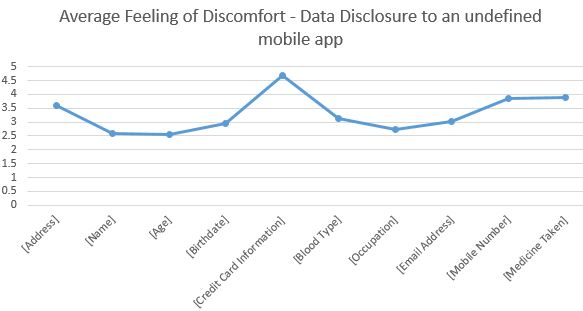
\includegraphics[width=0.5\textwidth]{Average_Generic}
\caption{Feeling of Discomfort in Disclosure - Undefined application}
\end{center}
\end{figure}

\begin{figure}[h]
\begin{center}
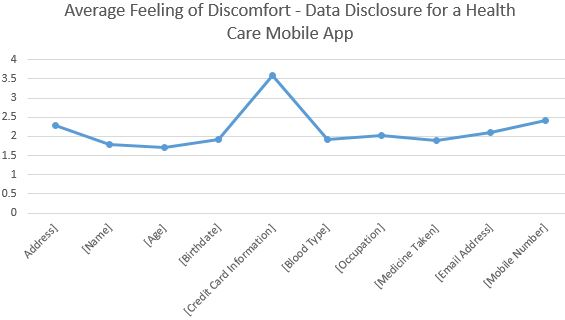
\includegraphics[width=0.5\textwidth]{Average_Health}
\caption{Feeling of Discomfort in Disclosure - Health  application}
\end{center}
\end{figure}

\begin{figure}[h]
\begin{center}
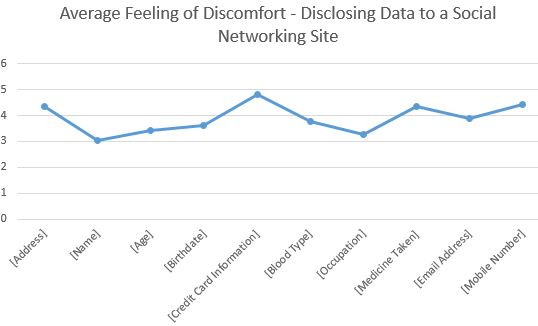
\includegraphics[width=0.5\textwidth]{Average_SocialNetworking}
\caption{Feeling of Discomfort in Disclosure - Social Networking application}
\end{center}
\end{figure}

\begin{figure}[h]
\begin{center}
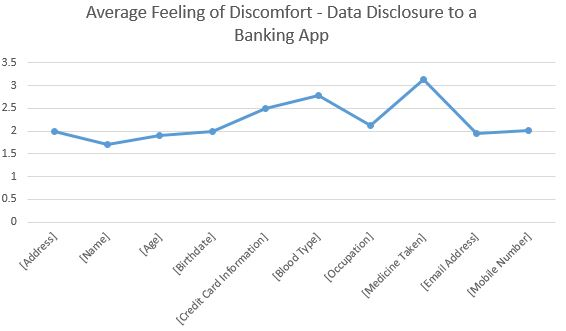
\includegraphics[width=0.5\textwidth]{Average_Banking}
\caption{Feeling of Discomfort in Disclosure - Banking application}
\end{center}
\end{figure}

It can be seen that irrespective of the context of disclosure, participants had a higher discomfort in disclosing their credit card number. This is because users consider their credit card number to be a highly sensitive data item.  Similarly we observed higher discomfort in disclosing medicine taken and blood type. However, the discomfort in disclosing the credit card number was very low for banking app because the credit card number is a data item that is relevant for the banking app. This suggests that users feel more comfortable sharing even sensitive data if the data item is relevant for the application. This observation is also observed with lowered discomfort in sharing medicine taken and blood type with a health care app.

Users demonstrated a relatively higher discomfort in sharing details with a social networking site. We defined the social networking site to have no control over data visibility once the data is disclosed. Therefore, we can assume that users have concern over data visibility when they disclose data into an application. 

In order to achieve the goals of the research, we calculate the effect of the variables we studies on the feeling of discomfort in disclosing data in the following subsections.

\subsection{Effect of data sensitivity to the feeling of disclosure -  $F_d,D_s$}

In order to calculate this we defined sensitive data from the 10 data items we provided the users following the definition for sensitive data in the data protection regulations [more details to be included]. We first calculated the feeling of disclosure of credit card\/name, blood type\/name and medicine taken\/name for all 151 participants and then averaged this across the 151 participants. Then we took the average of these three values as the average effect of sensitivity on data disclosure discomfort. The value we received was 1.840. Table 05 shows the values we calculated.

\begin{center}
\begin{table}[htbp]
\caption{Effect of Data Sensitivity when disclosing Data in the same application on disclosure discomfort}
\begin{center}
\begin{adjustbox}{width=0.4\textwidth}
\begin{tabular}{|l|l|}
\hline
Disclosing Sensitive Data &  Disclosing Age\\
\hline
Disclosing Credit Card Data & 2.399668874\\
\hline
Disclosing Medicine Taken & 1.971192053\\
\hline
Disclosing Mobile Number & 1.896909492\\
\hline
Disclosing Blood Type & 1.475496689\\
\hline
Disclosing Email Address & 1.458388521\\
\hline
\end{tabular}
\end{adjustbox}
\end{center}
\end{table}
\end{center}

THe hfindings also revealed that users were most sensitive about their credit card number followed by medicine they took. 

\subsection{Effect of data relatedness to the feeling of disclosure -  $F_d,D_r$}

In order to calculate the relatedness, we identified related data for the three application contexts we defined (disregarding the generic application context). We defined blood type to be related to the health care application, and medicine taken and blood type to be related to the health care app. We used the same data items in the social networking app as instances of disclosing unrelated data. The average effect of relatedness on data disclosure discomfort we received was 0.532, which suggests that users feel comfortable sharing data when the data item is related to the application. 

\subsection{Effect of data visibility to the feeling of disclosure -  $F_d,D_v$}

For this, we told the participants that the data visibility in the social networking app is not controllable for the user. That is they did not have control over who could see the data in the application. We also told them that the generic app had control for visibility. Then we compared the discomfort of sharing their age, address, email address and mobile number. We obtained the average effect of visibility on data disclosure discomfort as 2.66. This shows that users were more uncomfortable sharing their data in the event they had no control over the visibility over data. Compared to the other two factors (relatedness and sensitivity) users were most concerned about the visibility. 


\subsection {Relationship among sensitivity, visibility and relatedness}

We observed that participants were most concerned about the visibility their data get in an application when they disclose data. $F_d,D_v(av)$ had a value of 1.285, where as $F_d,D_s(av)$ had a value of 1.840. Both sensitivity and visibility of data were directly proportional to the discomfort of data disclosure (effect $>$ 1). 

visibility against sensitivity had an increased effect of 1.5. That is users were 1.5 times more uncomfortable sharing their data considering visibility than the sensitivity of the data.


As expected, the relatedness of a data item to the application context was observed to be inversely proportional to the discomfort in sharing data items. The average effect of relatedness on discomfort of disclosing data had a value of 0.531 (effect $<$ 1).

Therefore, we define the relationship of data sensitivity, visibility and relatedness to the privacy risk associated with the data item for a given software system context as below,

\[ \text{Privacy Risk}  =
\frac{
      \text{Sensitivity} \times 1.5 \times \text{Visibility} }
 {
       \text{Relatedness }}
\]

\subsection{Qualitative analysis on factors that affect the feeling of discomfort in data disclosure}

Table 05 gives the summary of the codes we generated through the qualitative analysis. We developed a totla of 11 codes.

\begin{center}
\begin{table*}[htbp]
\caption{Issues participants faced when embedding privacy into the designs}
\begin{center}
\begin{adjustbox}{width=1\textwidth}
\begin{tabular}{|p{0.20\linewidth}|p{0.64\linewidth}|p{0.16\linewidth}|}
\hline
Code &  Representative Quotes & Coverage (out of 151)\\
\hline
Benefit to me &how it benefits myself/ how useful it is for me. & 2.64\% (4)\\
\hline
How much I need the app &  ased on my requirements from the application & 7.2\%(11)\\
\hline
News I see  & by considering cyber crimes and all that & 0.66\%(1) \\
\hline
Personal experience &  I was in couple of these situations which gave me an idea & 2\%(3) \\
\hline
Personal Safety & Some data are highly confidential and could end up in a reputational and/or financial loss/  don't like to see unwanted advertisements and messages & 12\% (19)\\ 
\hline
Relevance of data to the purpose &if I don't think such applications needs the data. For instance my blood group for a banking app
 & 26\% (40)\\ 
\hline
Visibility of Data - who can see it & audience with access to the data/ as in whether I could control what others see & 12\% (19)\\ 
\hline
Sensitivity of Data & As long as the requested information is not sensitive/  some sensitive information can't be disclosed irrespective of the application
 & 15\% (23)\\ 
\hline
Transparency - knowing how the data is used & Depends on what they are going to do with the information/ when privacy is not guaranteed & 6.6\% (10)\\ 
\hline
Trust with the application & every online application cannot be trusted/ andom Facebook applications are not safe & 11\% (17)\\ 
\hline
Trust with the organization & If it is a reputed or a government institution there is less doubt and more trust on data security
 & 19\% (29)\\ 
\hline
\end{tabular}
\end{adjustbox}
\end{center}
\end{table*}
\end{center}

When it comes to data, participants mentioned only sensitivity, relevance and visibility of the data items that affect their disclosure decisions. Participants were most concerned about the relevance of data (26\%) followed by sensitivity of data (15\%) and visibility (12\%). Therefore, we could not identify any other factor related to data, that affects user disclosure decisions from the answers we received. 

However, we identified that users are concerned about the trust towards the organization that develop and publish applications (19\%). Participants said that they are comfortable sharing data as long as the application is developed and owned by a trusted organization. Some participants spoke about the trust with the application itself rather than the organization (11\%). Some particpants also raised concerns about personal safety (12\%). Their concerns on personal safety was two fold. One was on financial and reputational loss on data being accessed by unknown parties. The other was their concern on being subjected to unwanted marketing via phone and email. They said that they consider this as a personal threat and hence they think twoce before disclosing data to any application. A small number of participants were concerned about the previous personal experience and also about the benefit of sharing the data. 

\section{Discussion}

[to be decided]

\section {Limitations}

The study had several limitations. Firstly this was a remote survey. While remote surveys are beneficial in getting a large sample of participants in a relatively small period of time, direct engagement with users would disclose more in depth information when it comes to qualitative analysis. However, the main contribution of the paper was the derivation of the privacy measurement formula. Furthermore, for the qualitative component of data analysis we reached data saturation with the codes with 17 participants. The survey had 133 respondents which makes the results valid. Contextual studies involving real time applications that directly engage users in a natural setting could be used to observe how our findings stand in such setups.



\section{Conclusion and Future Work}




\iffalse

\begin{figure} 
\centering
\includegraphics [height=2 in,width=3 in]{Figure2.pdf}
\caption{Answer structure in a given security question \protect}
\vskip -6pt
\end{figure}
\fi

\iffalse 
Lying to a human being is a very bad thing to do, but, what if one lying to a computer to protect her privacy and keep her safe. 
\fi


\iffalse 
% no \IEEEPARstart
This demo file is intended to serve as a ``starter file''
for IEEE conference papers produced under \LaTeX\ using
IEEEtran.cls version 1.7 and later.
% You must have at least 2 lines in the paragraph with the drop letter
% (should never be an issue)
I wish you the best of success. 
\hfill mds
\hfill January 11, 2007

\subsection{Subsection Heading Here}
Subsection text here.


\subsubsection{Subsubsection Heading Here}
Subsubsection text here.
\fi




\iffalse 
\footnotesize
\bibliographystyle{abbrv}
\section{Conclusion}
The conclusion goes here. 




% conference papers do not normally have an appendix


% use section* for acknowledgement
\section*{Acknowledgment}


zzxzxz


\fi




\bibliographystyle{IEEEtran}
% argument is your BibTeX string definitions and bibliography database(s)
\bibliography{references}

\iffalse 
\begin{thebibliography}{1}

\bibitem{IEEEhowto:kopka}
H.~Kopka and P.~W. Daly, \emph{A Guide to \LaTeX}, 3rd~ed.\hskip 1em plus
0.5em minus 0.4em\relax Harlow, England: Addison-Wesley, 1999.

\end{thebibliography}




\section{Interview script}
Interview study 

\subsection*{ Demographics}

\begin{enumerate}
\item How old are you? ~\footnote{Most questions are open-ended questions}\\
\item How many people other than you live in your house?\\ 
\item What is each person's relationship to you?\\
\item What grade are you in school?\\
\end{enumerate}
\fi
\appendices

\section {Appendix A Survey Questionnaire}



% that's all folks
\end{document}



